\section{Physical effects}
\label{sec:physics}

Noise in tomography is unavoidable, and it makes segmentation harder because it further obscures the
boundaries between materials. Materials may be well separated from certain angles in the
3d-reconstructed image, but can overlap from others. Some noise like that corrected by flat-field
correction is very uniformly distributed across images. Other noise is however very spatially
dependent on its surrounding regions. Knowing the composition and positioning of the materials being
imaged, we can counter some of these effects during segmentation. The effects from noise manifest
themselves as numerical shifts in voxel-values as a function of their position. This is a direct
result of a misrepresented attenuation along the axis the X-rays are passing.

This dependency on orientation illustrates how voxel intensity values are not globally fixed.
Instead, how a certain material is represented in intensity, is highly dependent on its position
relative to neighbouring regions. Especially since this also determines the amount and type of
derived noise.  The same material with the same density, can thus be represented at multiple varying
intensities within the same sample.

% \begin{figure*} \centering 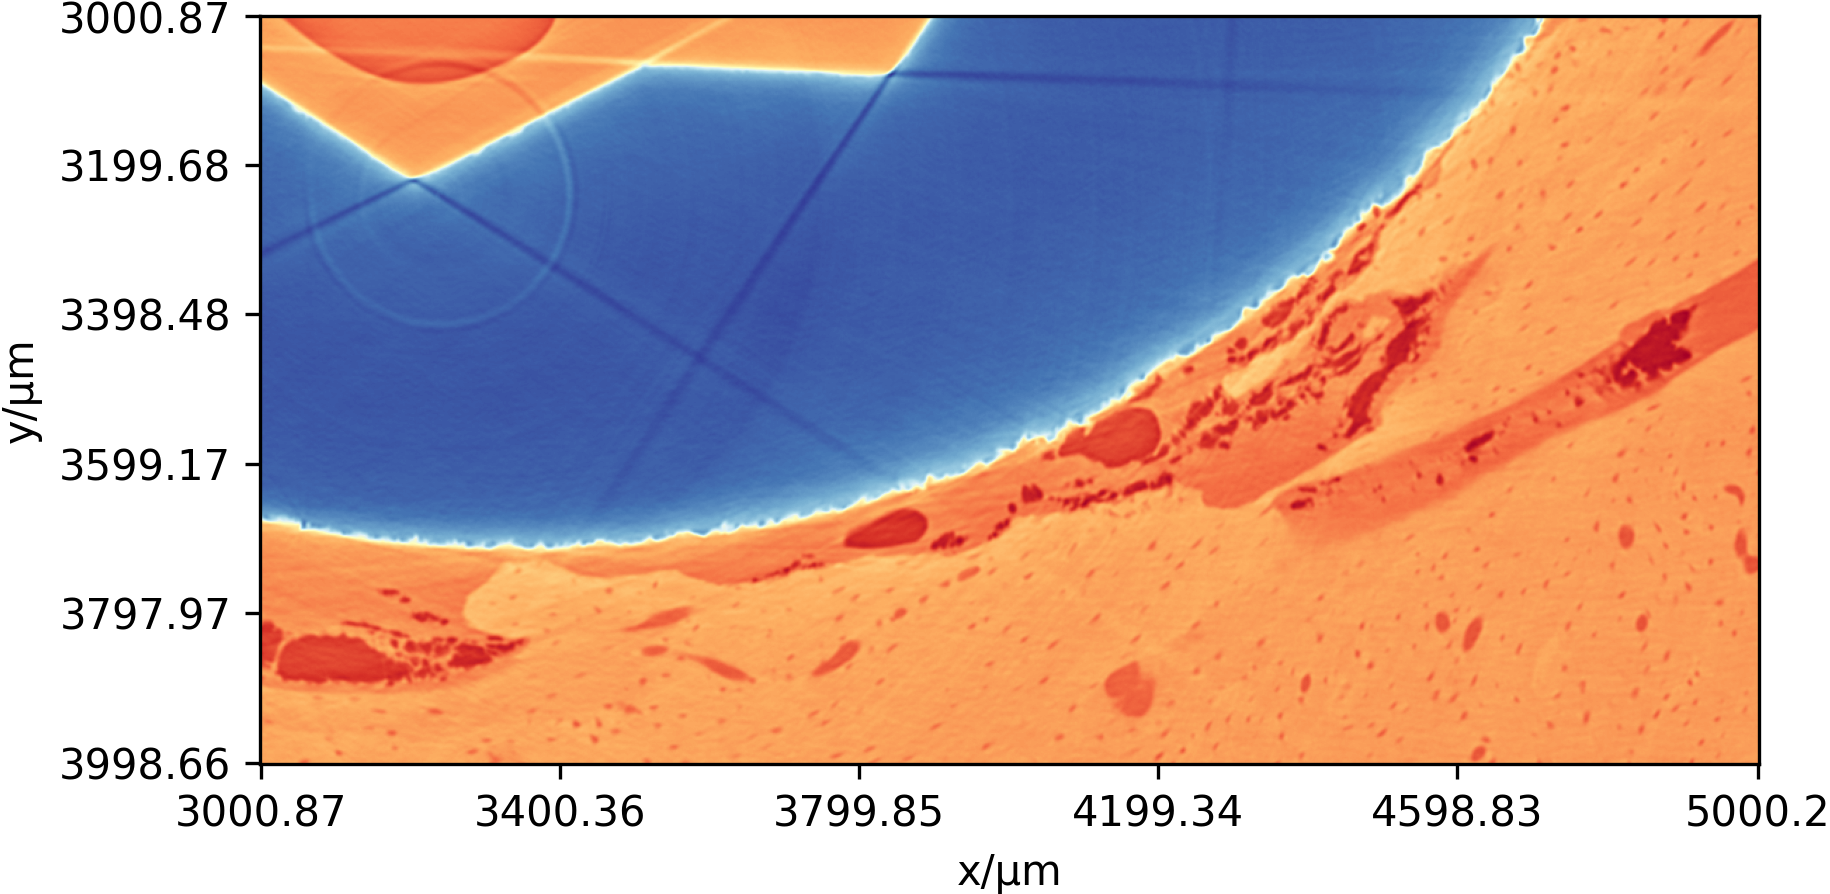
\includegraphics[width=\textwidth]{770c_pag-bic-xy-1x.png}
% \caption{Here we see a 1mm x 2mm region of an unscaled image slice in the XY dimension. It
% highlights some of the imperfections and noise present in the data. We especially see artifacts
% within and around the titanium implant.} \label{fig:xy-slice} \end{figure*}

\begin{figure}
  \centering
  \begin{tabular}{cc}
    \!\!\!\!\!\!(a)\!\!\!&\begin{tabular}{c}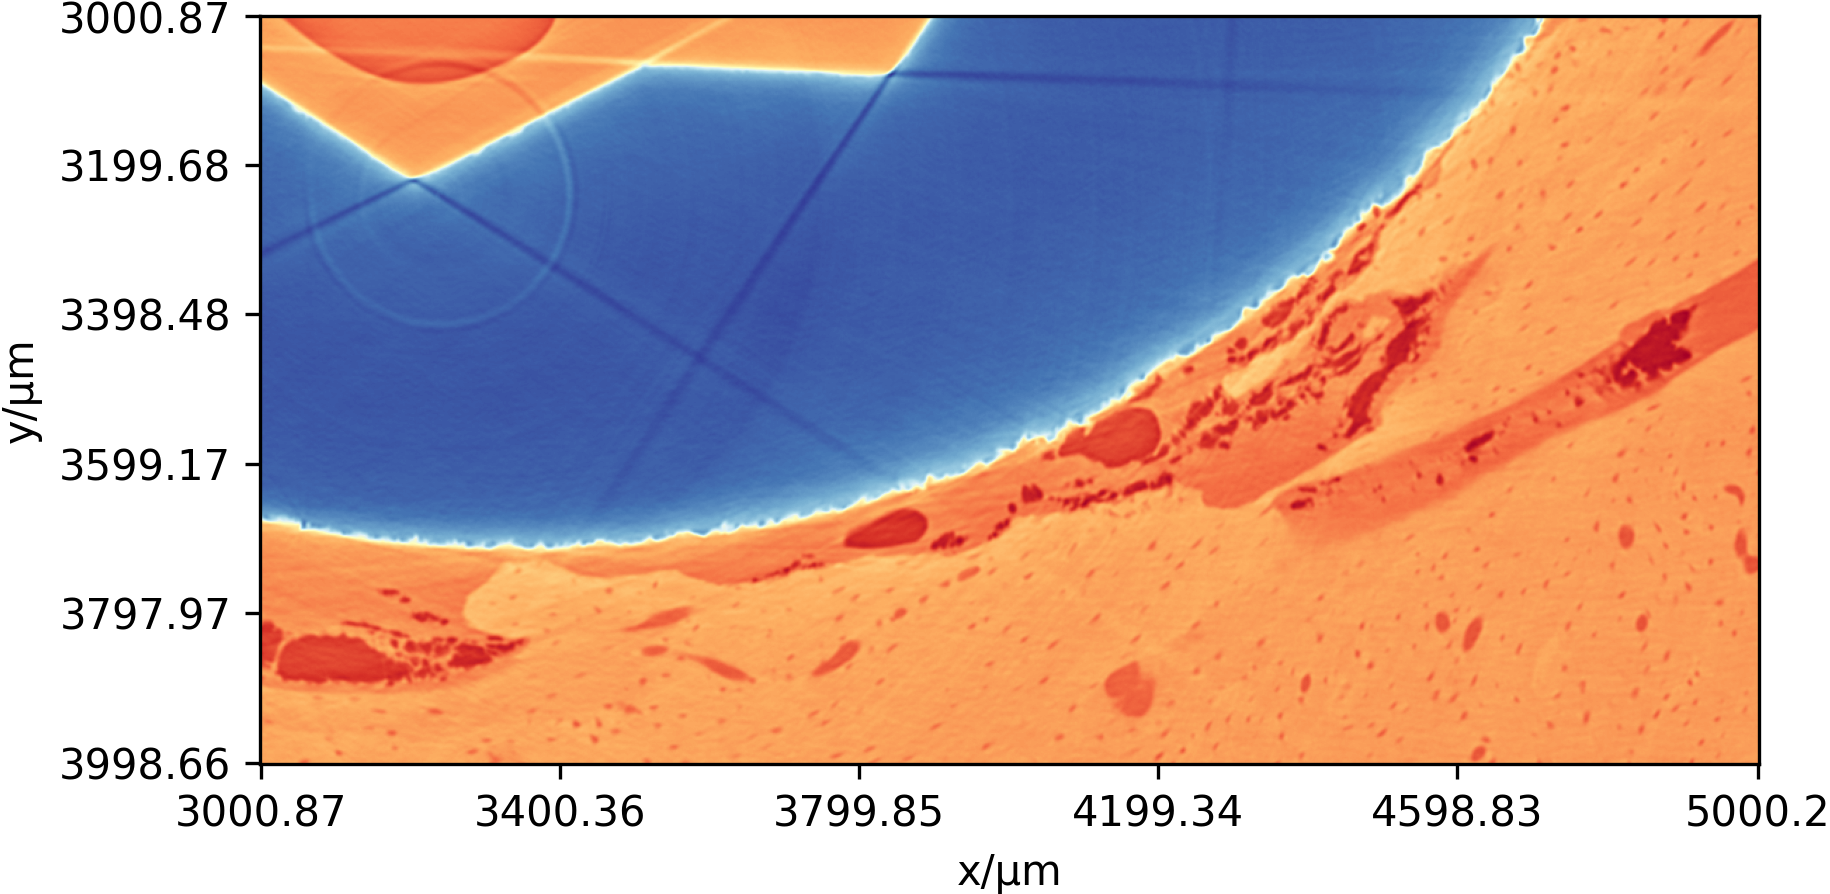
\includegraphics[width=0.96\columnwidth]{770c_pag-bic-xy-1x.png}\end{tabular}\\
    \!\!\!\!\!\!(b)\!\!\!&\begin{tabular}{c}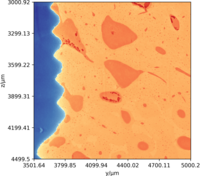
\includegraphics[width=0.96\columnwidth]{770c_pag-bic-yz-1x.png}\end{tabular}\\    
  \end{tabular}
  \caption{
    To better see the distortion effects, we zoom in on sub-regions of the slices shown in
    \Cref{fig:3viewsample}. Our visual systems automatically correct for most of the distortions,
    as they appear similar to illumination effects. However, even some distance from the implant,
    blood vessel voxels have higher values than bone voxels further out. As we approach the implant,
    the value-shifts accelerates and becomes highly non-linear.
    (a) A 1mm$\times$2mm region of an image slice in the XY-plane.
    % It highlights some of the imperfections and noise present in the data.
    (b) A 1.5mm x 1.5mm region of an image slice in the YZ-plane in the micro threaded part of
    the titanium implant.
  }
\label{fig:slices}
\end{figure}

In \Cref{fig:slices}, we see zoomed in regions of the XY- and YZ-planes of the same sample as shown
in \Cref{fig:3viewsample}.  Both planes display a broad selection of the various type of noise
sources found in the data.

\paragraph{Beam hardening}
Medical CT and $\mu$CT both utilize poly-energetic beams, which can cause artefacts around high
density regions. This effect is called beam-hardening \citep{beam-hardening}, and occurs when rays
with lower energy are attenuated more frequently, thus shifting the remaining photon energy to a
higher effective average value. This offsets the local contrast, by overestimating the attenuation,
leaving lighter spots on the image. Many types of artefacts will typically be present in X-ray 
setups, but most are taken into account by calibration using phantoms and pre-hardening the beam
before it reaches the sample. Pre-hardening of the beam is done using filters that attenuate the
softest rays. Due to its common usage, various metal artefact reduction (MAR) software exists to
account for noise and imperfections during reconstruction \citep{mar1}\citep{mar2}.

Despite the practically mono-energetic rays from SR$\mu$CT, the source initially generates a
poly-chromatic spectrum. During monochromatisation the resulting spectrum can still contain
corrupted harmonic components. Only a few percent corruption is enough to produce strong artefacts,
although monochromatisation is typically done in multiple layers \citep{srnoise}.  It can not
trivially be rejected that some noise does occur from poly-energetic incident radiation.  Two
distinct effects typically seen as a result of beam-hardening are in dark and bright streaks and
cupping artefacts in high density regions.

\paragraph{Dark and bright streaks} Streaking artefacts occur at the dense implant region, but also
in the transition from bone to softer tissue. This effect is mostly seen in regions of large
heterogeneity. When X-ray beams pass at angles containing multiple dense obstacles, the beam is
hardened more. Then for angles with fewer dense obstacles the energy spectrum is preserved better.
This produced the dark and bright streaks seen in \Cref{fig:slices}.

For a hardened beam, softer x-rays are absorbed instead of successfully penetrating the object, and
will not contribute to image formation. High density structures such as the titanium implant break
the isotropy, making the projected X-ray mean energy spectrum dependent on incident orientation
\citep{srnoise}.

\paragraph{Cupping effect} A common artefact that occurs when beams pass more homogeneous
cylindrical objects. Since beams passing the middle will traverse more material compared to the
edges, the beam is hardened more towards the center and intensity becomes lower as a result. This
can manifest itself in what erroneously looks to be dense peripheral regions at the edges.

\paragraph{Phase contrast} Phase contrast is an effect whose consequences are not very unlike those
of beam-hardening.  Although used as an advantage in holotomography\citep{holotomography} and phase
contrast tomography\citep{phasecontrast}, it induces noise in regular tomography such as used here.
It typically results in fringes around edges of regions within the image\citep{srnoise}. Similar to
dark and bright streaks mentioned above, they show as misrepresentations of the voxel values. In our
case we see them especially at the transitional edges between the titanium implant and the
biological tissue and bone.

\subsection{Other noise and artifacts}
\label{sec:noise-artefacts}

\paragraph{Ring artefacts} Looking at the XY-place in \Cref{fig:slices} we see clear concentric ring
artefacts emanating from the center of the sample, and at strong edges of the titanium implant. It
propagates strongly through the large region of air behind the implant. Compared to the other
artefacts mentioned, this effect is arising from imperfections in the scanner setup. These types of
artefacts can typically come from uncalibrated or defect adjacent detector elements. For synchrotron
radiation sources it can also occur from shifts and vibrations in the monochromator crystal
\citep{ringartefacts}.

\paragraph{Projection artefacts} Bright streaks with strong edges are seen from the sharp corners of
the titanium implant. When doing back projection, a symmetry break is seen as smeared lines across
the sample. This can occur from the high pass filter used during filtered back projection, which
exaggerates the differences between adjacent elements \citep{ctnoise}.

\paragraph{Compton scattering} Lower energy rays contribute mostly with noise from scattering
effects. A ray will propagate through a material, get scattered and diffract from its initial
trajectory. This gives a misrepresentation of the attenuation along its initial trajectory. The
artefacts seen from scattering are similar in nature to those formed by beam hardening. This is
because both phenomena effectively reduce the measured attenuation. For energy levels relevant for
the data presented here, of 50 KeV and above, Compton scattering is the dominant type
\citep{Compton}.  The scattering occurs due to photon-electron interaction between X-ray beam and
the material it passes through. Like beam-hardening, scattering will cause dark streaks across the
image, where attenuation was highest.

\subsection{Dealing with artefacts}
\label{sec:dealwithit}

The distortions that come from the class of physical effects and noise artefacts discussed in this
section, will vary continously as a function of the spatial coordinates. This allows the possibility
for a method, which can correctly identify materials despite varying voxel values.
% FIXME: Would like a reference for the continous argument
% It is also mentioned in the last sentences of the first paragraph in
% "Physical effects, noise and artifacts"

%Partial volume artefacts which are dependent on the voxel size and are mentioned briefly by Neldam et al.


%%% Local Variables:
%%% mode: latex
%%% TeX-master: "main"
%%% End:
